\documentclass[11pt,a4paper]{article}
\usepackage[T1]{fontenc}
\usepackage[utf8]{inputenc}
\usepackage[italian,provide=*]{babel}
\usepackage{mathptmx,microtype}
\usepackage[margin=2.5cm]{geometry}
\usepackage{amsmath,amssymb}
\usepackage{graphicx,booktabs,caption,array}
\usepackage[hidelinks]{hyperref}
\captionsetup{font=small,labelfont=bf}
\graphicspath{{figure/}}
\setlength{\parskip}{0.35em}
\title{\emph{Volatility risk premium} e strategie non direzionali\\ in opzioni sull'indice S\&P 500:\\ evidenza dalle \emph{option chain} SPX 2010--2023\thanks{Autori: Giordano Margotti, Alex Crescentini, Alessandro Celani, Giulio Sciacchitano (gruppo di lavoro \emph{finance-thinking}, repository \texttt{options\_strategy}). Le analisi di questo documento sono state ricalcolate integralmente sulle \emph{option chain}; errori e omissioni restano degli autori. Il documento ha finalità di ricerca e non costituisce consulenza in materia di investimenti.}}
\author{}
\date{Novembre 2026}
\begin{document}
{\let\newpage\relax\maketitle}
\vspace{-3em}

\begin{abstract}
\noindent Il lavoro verifica, sulle \emph{option chain} giornaliere delle opzioni europee sull'indice S\&P 500 (SPX) dal 2010 al 2023 (3.499 sedute, 47.699 coppie data--scadenza), se esista un \emph{volatility risk premium} (VRP) e se le strategie non direzionali di vendita di opzioni riescano a incassarlo al netto dei costi. La risposta dipende dalla misura adottata. La volatilità implicita \emph{model-free} a 30 giorni supera la volatilità successivamente realizzata di +3{,}45 punti in media (statistica $t$ 6{,}48), mentre la volatilità implicita \emph{at-the-money} la supera di soli +0{,}72 punti ($t$ 1{,}36): il premio risiede nelle code della distribuzione, in particolare nelle put \emph{out-of-the-money}, non nel livello centrale della superficie. Il premio \emph{at-the-money} è significativo nel 2010--2014 e statisticamente nullo nei due sottoperiodi successivi. Su 434 configurazioni di dieci famiglie di strategie (1.310.509 operazioni simulate), l'indice di Sharpe mediano è +0{,}39 ai prezzi mid e $-$0{,}40 ai prezzi bid-ask; la quota di configurazioni con alfa rispetto all'indice significativamente positivo passa dal 16{,}4\% al 2{,}5\%. I risultati positivi sono concentrati nelle strutture che vendono put e sono spiegati in larga parte dall'esposizione al mercato azionario. L'evidenza è coerente con un premio che esiste come compenso per il rischio di coda, ma che lo spread bid-ask e la selezione a posteriori dei parametri rendono difficilmente incassabile in modo sistematico.

\medskip\noindent\textbf{Parole chiave:} \emph{volatility risk premium}, volatilità implicita, opzioni su indice, iron condor, put credit spread, GJR-GARCH, costi di transazione, \emph{multiple testing}.
\end{abstract}

\section{Introduzione}

Il progetto da cui nasce questo documento ha per oggetto la possibilità di ottenere \emph{extra return} con strategie non direzionali in opzioni, ossia strategie il cui risultato non dipende dalla direzione del sottostante purché il prezzo resti entro un intervallo o la volatilità si mantenga contenuta. Si tratta di strategie di vendita di premio: iron condor, strangle, put credit spread e strutture affini. Il documento di impostazione del progetto individua tre fonti di rendimento atteso: la permanenza del prezzo in un intervallo, il decadimento temporale del valore delle opzioni e l'esistenza di un premio per il rischio di volatilità (\emph{volatility risk premium}, VRP), cioè di una differenza sistematica tra la volatilità implicita nei prezzi delle opzioni e la volatilità che il sottostante realizza in seguito.

Le prime due fonti non sono rendimenti attesi in senso proprio. Il decadimento temporale è il corrispettivo dell'esposizione alla convessità: in un mercato in cui le opzioni sono prezzate correttamente, il theta incassato compensa in media le perdite da gamma. La permanenza in un intervallo è già incorporata nel premio. L'unica fonte di rendimento atteso positivo per chi vende opzioni è quindi la terza: un prezzo delle opzioni superiore al valore atteso del loro payoff sotto la misura reale. La domanda di ricerca è di conseguenza duplice:
\begin{enumerate}
\item il premio per il rischio di volatilità esiste nei dati, con quale ampiezza, in quale regione della superficie di volatilità e con quale stabilità nel tempo;
\item le strategie non direzionali esaminate dal progetto riescono a incassarlo, tenuto conto dello spread bid-ask, delle commissioni, del margine e del numero di configurazioni provate.
\end{enumerate}

Il contributo del documento è empirico. Tutte le statistiche sono calcolate sulle quotazioni di fine giornata delle opzioni SPX dal 4 gennaio 2010 al 29 dicembre 2023, con un impianto volutamente semplice e riproducibile: volatilità implicita ricavata dai prezzi con il modello di Black (1976) sul forward implicito nella \emph{put-call parity}, varianza implicita \emph{model-free} con la formula del Cboe, varianza realizzata fino alla scadenza della stessa opzione, previsione GJR-GARCH(1,1) con innovazioni $t$ di Student stimata su \emph{expanding window} senza uso di informazioni future. Il codice e i risultati sono pubblicati nel repository insieme a un sito interattivo che consente di esplorare ogni configurazione.

Il documento è organizzato come segue. La Sezione~\ref{sec:lett} riassume la letteratura sull'esistenza, sulle cause e sulla persistenza del premio. La Sezione~\ref{sec:dati} descrive dati e metodo. La Sezione~\ref{sec:vrp} presenta l'evidenza sul premio; la Sezione~\ref{sec:strat} i backtest delle strategie; la Sezione~\ref{sec:rob} i controlli di robustezza e la correzione per \emph{multiple testing}. La Sezione~\ref{sec:codice} documenta le verifiche sul codice preesistente. Le Sezioni~\ref{sec:limiti} e~\ref{sec:concl} discutono limiti e conclusioni.

\section{Letteratura}\label{sec:lett}

\subsection{Definizione ed evidenza}

Il premio per il rischio di varianza è la differenza tra il valore atteso della varianza futura sotto la misura \emph{risk-neutral} e il suo valore atteso sotto la misura reale. Il primo termine è osservabile: Britten-Jones e Neuberger (2000) mostrano che la varianza attesa \emph{risk-neutral} è replicabile con un portafoglio statico di opzioni su tutti gli strike, senza ipotesi sul modello; Jiang e Tian (2005) ne studiano il contenuto informativo e l'indice VIX ne è l'implementazione di mercato. Carr e Wu (2009) costruiscono tassi di \emph{variance swap} sintetici per indici e singoli titoli e documentano che, per gli indici azionari statunitensi, la varianza implicita supera sistematicamente quella realizzata: chi vende varianza incassa un premio medio ampio e statisticamente significativo. Bakshi e Kapadia (2003) giungono alla stessa conclusione con una strategia diversa, mostrando che il guadagno di un'opzione acquistata e coperta in delta è in media negativo. Coval e Shumway (2001) trovano rendimenti medi fortemente negativi per gli straddle a delta nullo, e Bondarenko (2014) quantifica il costo storico delle put sull'indice: perdite medie mensili dell'ordine di alcune decine di punti percentuali per le put \emph{out-of-the-money}. Bollerslev, Tauchen e Zhou (2009) mostrano inoltre che la differenza tra varianza implicita e realizzata prevede i rendimenti azionari a orizzonte trimestrale, il che la qualifica come misura del prezzo del rischio e non come semplice errore di previsione.

\subsection{Perché il premio esisterebbe}

Le spiegazioni proposte appartengono a tre gruppi.

\emph{Compenso per un rischio sistematico.} La varianza aumenta quando i mercati scendono; un titolo che paga in quegli stati ha valore assicurativo e chi lo vende deve essere remunerato. Bates (2000) documenta che, dopo il crollo del 1987, i prezzi delle opzioni incorporano stabilmente il timore di salti negativi. Todorov (2010) e Bollerslev e Todorov (2011) attribuiscono la parte prevalente del premio alla compensazione per il rischio di salto, cioè alle code, più che alla volatilità diffusiva. Dew-Becker, Giglio, Le e Rodriguez (2017) mostrano che il prezzo del rischio è concentrato sulla varianza realizzata a brevissimo termine, mentre le notizie sulla varianza futura hanno prezzo prossimo a zero.

\emph{Domanda di copertura e vincoli degli intermediari.} Bollen e Whaley (2004) collegano la forma dello \emph{smile} di volatilità alla pressione netta degli acquisti di put sull'indice. Gârleanu, Pedersen e Poteshman (2009) costruiscono un modello in cui gli intermediari non possono coprirsi perfettamente e la domanda finale sposta i prezzi delle opzioni in proporzione al rischio non copribile. In questo schema il premio è il compenso di chi fornisce capacità di bilancio, e varia con essa.

\emph{Preferenze e percezioni.} Jackwerth (2000) ricava dalle opzioni un'avversione al rischio implicita incompatibile con preferenze standard dopo il 1987; Ilmanen (2012) riassume l'evidenza secondo cui, tra le classi di attivo, la vendita di assicurazione contro le code è stata remunerata e l'acquisto di esposizioni tipo lotteria è stato penalizzato.

\subsection{La posizione di efficienza}

La presenza di un premio medio positivo non contraddice l'efficienza dei mercati nel senso di Fama (1970): un rendimento atteso positivo a fronte di un rischio sistematico è un prezzo di equilibrio, non un'anomalia. La questione rilevante è se il premio ecceda il compenso giustificato dal rischio e se sia incassabile.

Su entrambi i punti la letteratura offre argomenti di cautela. Broadie, Chernov e Johannes (2009) mostrano che rendimenti medi molto negativi delle put non sono, da soli, evidenza di errore di prezzo: modelli standard con volatilità stocastica e salti generano rendimenti di quell'ordine, e i campioni disponibili sono troppo brevi per distinguere un premio elevato dall'assenza, nel campione, degli eventi rari che lo giustificano. Santa-Clara e Saretto (2009) mostrano che i requisiti di margine e i costi di transazione riducono drasticamente i rendimenti effettivamente ottenibili dalla vendita di opzioni: un investitore deve detenere molta liquidità per sopravvivere alle richieste di margine, e la strategia realizzabile è una frazione di quella teorica. Constantinides, Jackwerth e Savov (2013) documentano che i fattori di rischio usuali non spiegano i rendimenti delle opzioni su indice senza l'aggiunta di fattori specifici di salto e volatilità. Jurek e Stafford (2015) mostrano che il profilo di rendimento di molti fondi alternativi è replicabile con la vendita di put su indice e che, valutato al costo del capitale appropriato per quel rischio di coda, l'alfa apparente scompare. Israelov e Nielsen (2015) scompongono il rendimento delle strategie \emph{covered call} in esposizione azionaria, esposizione corta alla volatilità e \emph{timing} involontario, e mostrano che gran parte del rendimento è beta azionario.

Sul piano previsivo, la letteratura più recente ha rivalutato la volatilità implicita. Canina e Figlewski (1993) non trovavano alcun contenuto informativo; Christensen e Prabhala (1998), con campioni non sovrapposti, mostrano che la volatilità implicita è una previsione quasi non distorta ed efficiente della volatilità realizzata; la rassegna di Poon e Granger (2003) conferma che la volatilità implicita batte in genere i modelli di serie storiche.

Infine, il premio non è costante. Dew-Becker e Giglio (2023, 2025) documentano che negli ultimi quindici anni gli alfa delle opzioni su indice sono diventati statisticamente indistinguibili da zero e che il premio per il rischio di varianza si è ridotto, in coerenza con un modello in cui i prezzi delle opzioni sono determinati dagli intermediari e il costo della copertura è diminuito. Per le opzioni a scadenza giornaliera, Beckmeyer, Branger e Gayda (2023) stimano che gli investitori al dettaglio abbiano perso in aggregato sulle opzioni SPX con scadenza in giornata, in larga parte a causa dei costi di negoziazione.

\subsection{Implicazioni per il progetto}

Dalla letteratura discendono quattro previsioni verificabili sui dati disponibili: (i) il premio misurato con la varianza \emph{model-free} deve risultare maggiore di quello misurato sulla volatilità \emph{at-the-money}, perché la parte prevalente è compenso per le code; (ii) la distribuzione del premio realizzato deve essere fortemente asimmetrica a sinistra; (iii) il premio deve risultare più debole nella parte recente del campione; (iv) i rendimenti delle strategie di vendita devono ridursi sensibilmente una volta considerati i costi e l'esposizione al mercato azionario. Le sezioni seguenti le verificano una per una.

\section{Dati e metodo}\label{sec:dati}

\subsection{Dati}

La fonte è OptionsDX (\url{https://www.optionsdx.com}), dataset \emph{SPX Option Chains} con frequenza \emph{end-of-day}: file mensili \texttt{spx\_eod\_AAAAMM} dal gennaio 2010 al dicembre 2023, acquisiti tramite il repository del gruppo di lavoro. Ogni file contiene l'intera \emph{option chain} di ciascuna seduta alla chiusura, con una riga per coppia scadenza--strike e, per ciascun lato, bid, ask, volume, volatilità implicita e greche calcolate dal fornitore, oltre al livello del sottostante.

Lo strumento è l'opzione sull'indice S\&P 500 quotata al Cboe Options Exchange (\emph{ticker} SPX): opzione su indice di stile europeo, \emph{cash-settled}, con moltiplicatore pari a 100 dollari per punto indice. L'archivio comprende le scadenze mensili standard del terzo venerdì, \emph{AM-settled}, e le scadenze settimanali e di fine mese (SPXW), \emph{PM-settled}. L'archivio contiene 3.499 sedute; la sola interruzione superiore a cinque giorni di calendario cade nel gennaio 2011. Per le analisi si usano le scadenze con vita residua tra 1 e 75 giorni di calendario. Il livello dell'indice è quello riportato nelle \emph{option chain} alla chiusura.

I risultati in dollari si riferiscono a un contratto SPX; per il contratto XSP, di dimensione pari a un decimo, i valori si dividono per dieci, mentre le commissioni per contratto restano invariate e pesano quindi dieci volte di più in termini relativi.

\subsection{Forward, volatilità implicita e delta}

Per ogni coppia data--scadenza il forward implicito $F$ si ricava dalla \emph{put-call parity} sullo strike in cui i prezzi mid di call e put sono più vicini: $F = K^\ast + C(K^\ast) - P(K^\ast)$. In questo modo dividendi e tassi entrano tramite il mercato e non richiedono ipotesi esterne; il fattore di sconto sul premio, trascurabile sulle scadenze considerate, è posto pari a uno. La volatilità implicita di ciascuna opzione è ottenuta invertendo per bisezione la formula di Black (1976) sul prezzo mid, con $T$ pari ai giorni di calendario diviso 365; il delta è quello forward dello stesso modello. La volatilità \emph{at-the-money} è l'interpolazione lineare in strike, nel punto $K=F$, delle volatilità delle opzioni \emph{out-of-the-money}.

I controlli di integrità danno i risultati attesi: l'inversione riproduce i prezzi con errore massimo dell'ordine di $10^{-5}$ punti indice; al punto $K=F$ la volatilità implicita della put e quella della call coincidono (differenza mediana nulla, 5° e 95° percentile entro un decimo di punto di volatilità); il delta della call meno il delta della put vale uno; il costo di \emph{carry} implicito nel forward è coerente con il livello dei tassi al netto dei dividendi anno per anno.

\subsection{Varianza implicita model-free}

La varianza implicita \emph{model-free} segue la formula dell'indice VIX applicata alla singola scadenza:
\begin{equation}
\sigma^2_{\mathrm{MF}} = \frac{2}{T}\sum_i \frac{\Delta K_i}{K_i^2}\, Q(K_i) - \frac{1}{T}\left(\frac{F}{K_0}-1\right)^2 ,
\end{equation}
dove $Q(K_i)$ è il prezzo mid dell'opzione \emph{out-of-the-money} di strike $K_i$, $K_0$ è il primo strike non superiore a $F$ e la somma si arresta, su ciascun lato, dopo due bid nulli consecutivi. La media di $\sigma_{\mathrm{MF}}$ sulla scadenza più vicina a 30 giorni è 18{,}06\%, in linea con l'ordine di grandezza dell'indice VIX nel periodo.

\subsection{Varianza realizzata e definizione del premio}

Per un'opzione osservata in $t$ con scadenza in $t+T$, la varianza realizzata è la somma dei quadrati dei rendimenti logaritmici giornalieri dalla seduta successiva a $t$ fino alla scadenza, divisa per $T$ in anni di calendario:
\begin{equation}
RV_{t,T} = \frac{1}{T}\sum_{s=t+1}^{t+T} r_s^2 .
\end{equation}
Implicita e realizzata sono così annualizzate sullo stesso intervallo di calendario e si riferiscono esattamente allo stesso periodo. Il premio è riportato in tre forme: in punti di volatilità sulla misura \emph{at-the-money}, $\sigma_{\mathrm{ATM}} - \sqrt{RV}$; in punti di volatilità sulla misura \emph{model-free}, $\sigma_{\mathrm{MF}} - \sqrt{RV}$; in unità di varianza, $\sigma^2_{\mathrm{MF}} - RV$, che corrisponde al payoff di un \emph{variance swap} venduto.

Per ciascun orizzonte obiettivo (7, 14, 21, 30, 45 e 60 giorni) si seleziona, in ogni seduta, la scadenza con vita residua più vicina all'obiettivo entro una tolleranza prefissata. Poiché le osservazioni giornaliere si sovrappongono, gli errori standard sono di tipo Newey e West (1987) con numero di ritardi pari a una volta e mezza l'orizzonte in sedute; a verifica si riportano anche le statistiche sul campione non sovrapposto.

\subsection{Previsione GJR-GARCH}

Il modello di riferimento per la volatilità attesa sotto la misura reale è il GJR-GARCH(1,1) di Glosten, Jagannathan e Runkle (1993) con innovazioni $t$ di Student, generalizzazione asimmetrica dei modelli di Engle (1982) e Bollerslev (1986):
\begin{equation}
\sigma^2_{t+1} = \omega + \left(\alpha + \gamma\,\mathbf{1}_{\{\varepsilon_t<0\}}\right)\varepsilon_t^2 + \beta\,\sigma_t^2 .
\end{equation}
La stima usa un'\emph{expanding window} di almeno 504 sedute e viene ripetuta ogni 21 sedute; tra una stima e la successiva la varianza condizionata è aggiornata con i parametri correnti e con i soli rendimenti già osservati. La previsione della varianza totale fino alla scadenza è la somma delle previsioni giornaliere sulle $n$ sedute residue, $\sum_{k=1}^{n}\left[\bar\sigma^2 + p^{\,k-1}(\sigma^2_{t+1}-\bar\sigma^2)\right]$, con persistenza $p=\alpha+\gamma/2+\beta$ e varianza di lungo periodo $\bar\sigma^2=\omega/(1-p)$, annualizzata sullo stesso tempo di calendario dell'implicita. Non è applicato alcun fattore correttivo. Le previsioni sono disponibili dal gennaio 2012. Nei parametri stimati $\alpha$ risulta nullo e $\gamma$ compreso tra 0{,}24 e 0{,}36: nel campione la varianza reagisce soltanto ai rendimenti negativi.

\subsection{Disegno dei backtest}

In ogni seduta e per ciascuna scadenza obiettivo (7, 14, 30 e 45 giorni) viene aperta una posizione unitaria per ciascuna configurazione. Gli strike sono scelti per delta (0{,}10, 0{,}16, 0{,}20 e 0{,}30 per le gambe vendute); le \emph{wing} delle strutture a rischio definito seguono due regole alternative: delta 0{,}05 oppure distanza pari all'1\% dello spot. Le famiglie sono dieci: short put, short strangle, short straddle \emph{at-the-money}, put credit spread, call credit spread, iron condor, iron butterfly, long put, debit put spread e long calendar \emph{at-the-money}. Per le strutture a credito si considerano tre gestioni: mantenimento fino a scadenza; chiusura al raggiungimento di un profitto pari al 50\% del credito; chiusura al 50\% di profitto oppure a una perdita pari al 200\% del credito. Le condizioni di uscita sono valutate sui prezzi mid di chiusura giornaliera. In totale le configurazioni sono 434 e le operazioni simulate 1.310.509.

\emph{Prezzi di esecuzione.} Per ogni operazione si registrano il risultato ai prezzi mid e la somma dei \emph{half-spread} bid-ask delle gambe negoziate, in apertura e nell'eventuale chiusura anticipata. Il risultato è quindi una funzione lineare della quota $x$ di spread pagata: $x=0$ corrisponde ai prezzi mid, $x=1$ alla vendita al bid e all'acquisto all'ask. A scadenza il \emph{cash settlement} non comporta spread. La commissione è di un dollaro per gamba e per contratto.

\emph{Margine e rendimento.} Per le strutture a rischio definito il margine è la perdita massima; per le posizioni scoperte è il 20\% del valore nozionale, come nel codice del gruppo; per le strutture a debito è il premio pagato. Il rendimento di ogni operazione è il risultato diviso per il margine. Per ottenere una serie mensile confrontabile tra scadenze diverse si ipotizza un \emph{ladder} a capitale costante: il capitale è ripartito in parti uguali tra le posizioni contemporaneamente aperte, sicché ogni operazione contribuisce al rendimento del mese di chiusura per il proprio rendimento sul margine diviso per il numero di sedute dell'orizzonte. Le serie mensili sono sommate senza capitalizzazione; rendimento medio e \emph{drawdown} massimo scalano quindi linearmente con la quota di capitale impegnata a margine, mentre l'indice di Sharpe non ne dipende.

\emph{Esposizione al mercato.} Per ciascuna configurazione si stima la regressione dei rendimenti mensili sui rendimenti mensili dell'indice; l'intercetta annualizzata (alfa) misura il rendimento non spiegato dall'esposizione azionaria.

\section{Il premio per il rischio di volatilità nei dati}\label{sec:vrp}

\subsection{Livello medio per orizzonte}

La Tabella~\ref{tab:oriz} riporta, per ciascun orizzonte, la media della volatilità implicita \emph{at-the-money}, della volatilità \emph{model-free} e della volatilità realizzata, con le due misure del premio.

\begin{table}[ht]\centering\small
\caption{Volatilità implicita e realizzata per orizzonte, SPX 2010--2023. Valori in punti percentuali di volatilità annualizzata; $t$ con errori standard Newey-West.}\label{tab:oriz}
\begin{tabular}{rrrrrrrrrrrr}\toprule
 & & \multicolumn{3}{c}{Medie} & \multicolumn{3}{c}{ATM $-$ realizzata} & \multicolumn{2}{c}{MF $-$ realizzata} & & \\ \cmidrule(lr){3-5}\cmidrule(lr){6-8}\cmidrule(lr){9-10}
Giorni & Sedute & ATM & MF & Real. & Media & $t$ & \% $>0$ & Media & $t$ & Skew. & Min. \\ \midrule
7 & 2.892 & 15{,}18 & 17{,}09 & 13{,}84 & +1{,}34 & 5{,}43 & 68 & +3{,}25 & 13{,}33 & $-$3{,}7 & $-$99 \\
14 & 3.018 & 14{,}98 & 17{,}25 & 14{,}10 & +0{,}88 & 2{,}48 & 69 & +3{,}15 & 8{,}98 & $-$4{,}9 & $-$90 \\
21 & 3.098 & 15{,}09 & 17{,}57 & 14{,}33 & +0{,}76 & 1{,}72 & 68 & +3{,}24 & 7{,}31 & $-$4{,}9 & $-$79 \\
30 & 3.134 & 15{,}32 & 18{,}06 & 14{,}60 & +0{,}72 & 1{,}36 & 69 & +3{,}45 & 6{,}48 & $-$5{,}0 & $-$77 \\
45 & 3.104 & 15{,}99 & 19{,}06 & 15{,}18 & +0{,}81 & 1{,}22 & 70 & +3{,}88 & 5{,}71 & $-$4{,}5 & $-$71 \\
60 & 3.250 & 16{,}30 & 19{,}57 & 15{,}34 & +0{,}96 & 1{,}27 & 73 & +4{,}23 & 5{,}50 & $-$4{,}1 & $-$64 \\
\bottomrule\end{tabular}\end{table}

Emergono tre fatti. Primo: la volatilità \emph{model-free} supera la realizzata di oltre tre punti a tutti gli orizzonti, con statistiche $t$ comprese tra 5{,}50 e 13{,}33. Secondo: la volatilità \emph{at-the-money} supera la realizzata di meno di un punto oltre i 14 giorni, e la differenza non è statisticamente diversa da zero a 21, 30, 45 e 60 giorni; il premio \emph{at-the-money} è significativo soltanto a 7 giorni (+1{,}34 punti, $t$ 5{,}43) e a 14 giorni (+0{,}88 punti, $t$ 2{,}48). Terzo: la distribuzione è fortemente asimmetrica. A 30 giorni la mediana del premio \emph{at-the-money} è +1{,}74 punti e il premio è positivo nel 69{,}1\% delle sedute, ma la \emph{skewness} è $-$5{,}0 e il valore minimo, nel febbraio 2020, è $-$77{,}5 punti. La media è la somma di molti piccoli guadagni e di poche perdite molto ampie (Figura~\ref{fig:serie}).

\begin{figure}[ht]\centering
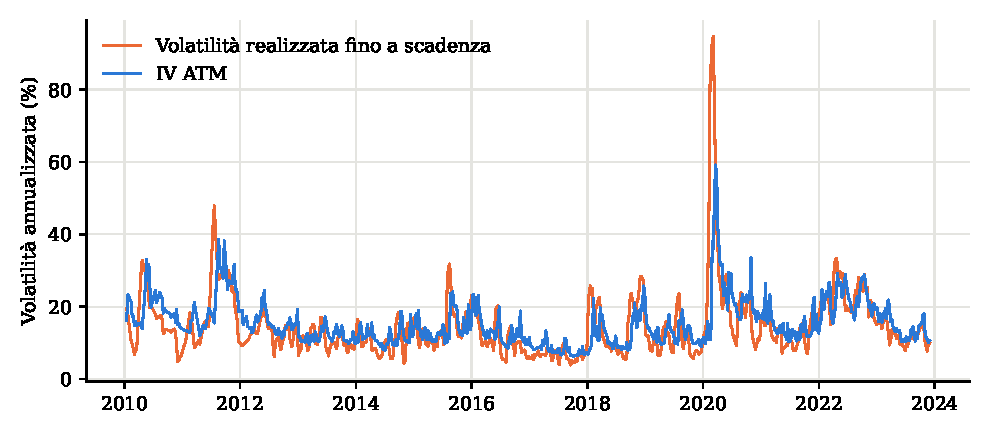
\includegraphics[width=\textwidth]{serie_it.pdf}
\caption{Volatilità implicita \emph{at-the-money} sulla scadenza più vicina a 30 giorni e volatilità realizzata fino a quella scadenza. Campionamento settimanale.}\label{fig:serie}
\end{figure}

La distanza tra le due misure implicite, circa 2{,}7 punti a 30 giorni, è il contributo delle \emph{wing} della superficie. Nel campione la volatilità implicita della put con delta 0{,}10 supera quella \emph{at-the-money} di 7{,}34 punti in media e la differenza tra put e call con delta 0{,}25 è di 5{,}48 punti. La prima previsione della letteratura è quindi confermata: il premio non è nel livello centrale della superficie, è nello \emph{skew}.

\begin{figure}[ht]\centering
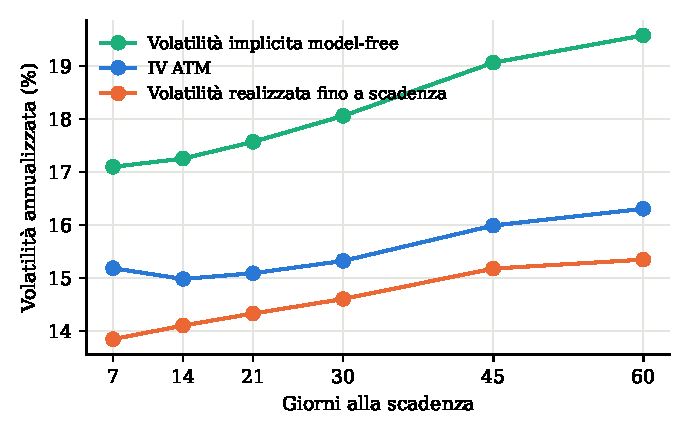
\includegraphics[width=0.48\textwidth]{struttura_it.pdf}\hfill
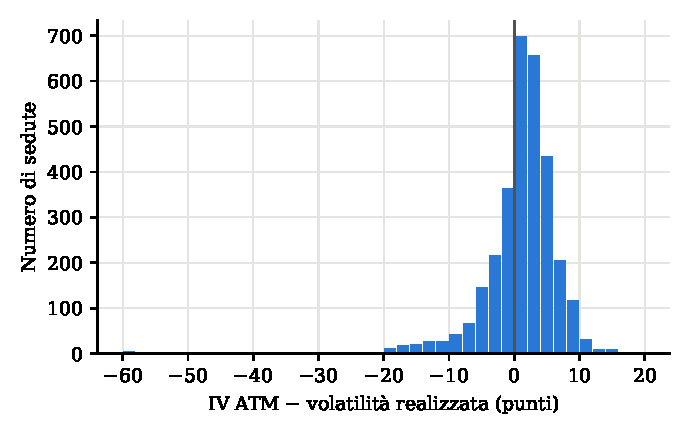
\includegraphics[width=0.48\textwidth]{isto_it.pdf}
\caption{A sinistra: medie per orizzonte delle tre misure di volatilità. A destra: distribuzione del premio \emph{at-the-money} a 30 giorni.}\label{fig:strut}
\end{figure}

\subsection{Stabilità nel tempo}

Il premio \emph{at-the-money} a 30 giorni vale in media +1{,}82 punti nel 2010--2014 ($t$ 4{,}02), +0{,}46 punti nel 2015--2019 ($t$ 0{,}84) e +0{,}04 punti nel 2020--2023 ($t$ 0{,}03). La Tabella~\ref{tab:anni} mostra il dettaglio annuale: quattro anni su quattordici hanno premio medio negativo (2015, 2018, 2020 e 2022) e sono gli anni in cui la volatilità realizzata è aumentata bruscamente. Il risultato è coerente con la riduzione del premio documentata da Dew-Becker e Giglio (2023, 2025), con l'avvertenza che tre sottoperiodi di pochi anni non consentono di distinguere una riduzione strutturale da una sequenza sfavorevole di eventi.

\begin{table}[ht]\centering\small
\caption{Premio \emph{at-the-money} a 30 giorni per anno. Valori in punti di volatilità.}\label{tab:anni}
\begin{tabular}{rrrrrrr}\toprule
Anno & Sedute & IV ATM & Realizzata & Premio & \% $>0$ & Minimo \\ \midrule
2010 & 108 & 19{,}96 & 15{,}86 & +4{,}09 & 83 & $-$19{,}0 \\
2011 & 104 & 21{,}66 & 21{,}22 & +0{,}45 & 65 & $-$32{,}3 \\
2012 & 187 & 15{,}65 & 12{,}71 & +2{,}94 & 90 & $-$1{,}8 \\
2013 & 252 & 12{,}39 & 10{,}82 & +1{,}57 & 70 & $-$4{,}6 \\
2014 & 249 & 11{,}89 & 11{,}06 & +0{,}83 & 60 & $-$8{,}2 \\
2015 & 252 & 14{,}47 & 14{,}84 & $-$0{,}37 & 62 & $-$20{,}6 \\
2016 & 251 & 13{,}60 & 11{,}39 & +2{,}21 & 79 & $-$7{,}9 \\
2017 & 250 & 8{,}32 & 6{,}69 & +1{,}64 & 82 & $-$3{,}0 \\
2018 & 252 & 13{,}08 & 16{,}01 & $-$2{,}93 & 49 & $-$17{,}2 \\
2019 & 247 & 12{,}95 & 11{,}16 & +1{,}79 & 77 & $-$12{,}9 \\
2020 & 250 & 24{,}66 & 27{,}12 & $-$2{,}45 & 64 & $-$77{,}5 \\
2021 & 246 & 14{,}89 & 12{,}68 & +2{,}22 & 73 & $-$6{,}6 \\
2022 & 256 & 22{,}56 & 23{,}75 & $-$1{,}19 & 43 & $-$17{,}9 \\
2023 & 230 & 14{,}60 & 12{,}81 & +1{,}79 & 83 & $-$2{,}7 \\
\bottomrule\end{tabular}\end{table}

\begin{figure}[ht]\centering
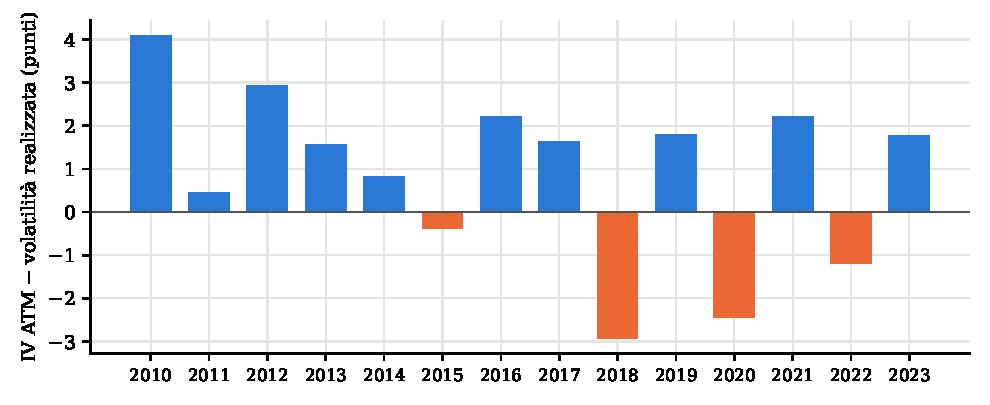
\includegraphics[width=0.85\textwidth]{anni_it.pdf}
\caption{Premio \emph{at-the-money} medio a 30 giorni per anno.}\label{fig:anni}
\end{figure}

\subsection{La volatilità implicita come previsione}

Se il mercato delle opzioni è efficiente sul piano informativo, la volatilità implicita deve essere una previsione non distorta della volatilità realizzata, a meno del premio per il rischio. La regressione di Mincer e Zarnowitz (1969), $\sqrt{RV_{t,T}} = a + b\,\sigma_t + u_t$, ne è la verifica standard: sotto l'ipotesi di previsione non distorta $a=0$ e $b=1$.

\begin{table}[ht]\centering\small
\caption{Regressioni di Mincer-Zarnowitz della volatilità realizzata sulla volatilità implicita. $a$ in punti di volatilità; valore $p$ del test congiunto $a=0$, $b=1$.}\label{tab:mz}
\begin{tabular}{rrrrrrrr}\toprule
 & \multicolumn{5}{c}{IV ATM} & \multicolumn{2}{c}{Model-free} \\ \cmidrule(lr){2-6}\cmidrule(lr){7-8}
Giorni & $a$ & $b$ & e.s. $b$ & $R^2$ & $p$ & $b$ & $p$ \\ \midrule
7 & $-$1{,}35 & 1{,}001 & 0{,}084 & 0{,}60 & 0{,}000 & 0{,}959 & 0{,}000 \\
14 & $-$1{,}34 & 1{,}031 & 0{,}109 & 0{,}55 & 0{,}001 & 0{,}981 & 0{,}000 \\
21 & $-$0{,}46 & 0{,}980 & 0{,}115 & 0{,}47 & 0{,}080 & 0{,}928 & 0{,}000 \\
30 & +0{,}69 & 0{,}908 & 0{,}099 & 0{,}39 & 0{,}409 & 0{,}841 & 0{,}000 \\
45 & +2{,}14 & 0{,}816 & 0{,}071 & 0{,}31 & 0{,}035 & 0{,}737 & 0{,}000 \\
60 & +3{,}08 & 0{,}752 & 0{,}072 & 0{,}25 & 0{,}002 & 0{,}662 & 0{,}000 \\
\bottomrule\end{tabular}\end{table}

A 30 giorni la pendenza stimata è 0{,}908 (errore standard 0{,}099) e l'ipotesi congiunta non è rifiutata ($p=$ 0{,}409): la volatilità \emph{at-the-money} è, nel campione, una previsione statisticamente non distorta. La stessa ipotesi è nettamente rifiutata per la misura \emph{model-free} a ogni orizzonte, come atteso per una misura che incorpora il premio per le code. A 7 e a 14 giorni la pendenza è prossima a uno e il rifiuto dell'ipotesi congiunta dipende dalla sola costante, cioè dal premio medio. Agli orizzonti di 45 e 60 giorni la pendenza scende sotto uno anche per la misura \emph{at-the-money}: la volatilità implicita elevata sovrastima la realizzata successiva.

\begin{figure}[ht]\centering
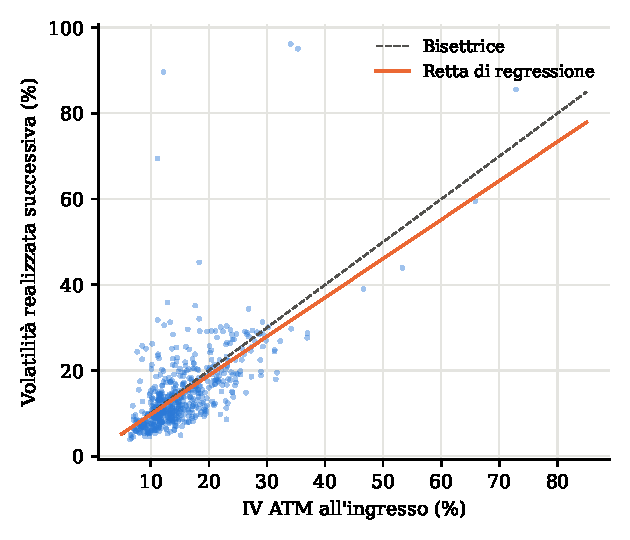
\includegraphics[width=0.46\textwidth]{mz_it.pdf}\hfill
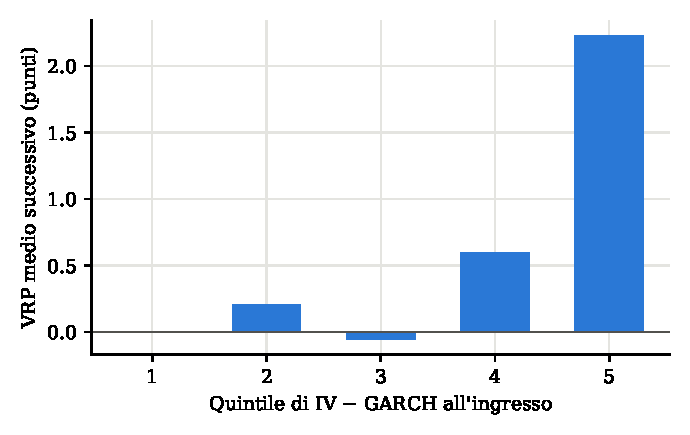
\includegraphics[width=0.50\textwidth]{gap_it.pdf}
\caption{A sinistra: volatilità realizzata contro volatilità implicita \emph{at-the-money} a 30 giorni. A destra: premio medio successivo per quintile della differenza tra volatilità implicita e previsione GJR-GARCH all'ingresso.}\label{fig:mz}
\end{figure}

Il confronto tra previsioni sul campione 2012--2023 (2.920 sedute, orizzonte 30 giorni) conferma la gerarchia nota in letteratura. L'errore quadratico medio è 7{,}38 punti per la volatilità \emph{at-the-money}, 8{,}15 per la \emph{model-free}, 8{,}26 per il GJR-GARCH e 9{,}22 per la volatilità storica a 21 sedute. Nella regressione che include le tre previsioni, il coefficiente della volatilità implicita è +0{,}73 ($t$ 6{,}50), quello del GJR-GARCH +0{,}27 ($t$ 1{,}77) e quello della volatilità storica $-$0{,}09 ($t$ $-$1{,}01), con $R^2$ pari a 0{,}41. Il modello GARCH aggiunge un'informazione marginale di significatività debole a quella già contenuta nei prezzi delle opzioni; la volatilità storica non ne aggiunge.

\subsection{Il segnale implicita meno GARCH}

Il progetto ha proposto come filtro di ingresso il confronto tra volatilità implicita e previsione GARCH. Ordinando le sedute in quintili della differenza $\sigma_{\mathrm{ATM}}-\sigma_{\mathrm{GARCH}}$, il premio medio successivo è +0{,}00, +0{,}21, $-$0{,}05, +0{,}60 e +2{,}23 punti dal primo al quinto quintile (Figura~\ref{fig:mz}). La relazione è crescente ed è concentrata nell'ultimo quintile; la regressione del premio successivo sulla differenza ha pendenza 0{,}21 con $t$ 1{,}55 e $R^2$ dell'1{,}5\%. Il segnale ha il segno atteso ma non raggiunge la significatività convenzionale.

\subsection{Il prezzo dell'assicurazione}

Una misura diretta del premio contenuto nelle put è il rapporto tra le perdite a scadenza e i premi incassati da chi le ha vendute (Tabella~\ref{tab:ins}). Un rapporto pari a uno corrisponde a un prezzo equo sotto la misura reale. Nel campione, per la put con delta 0{,}10 il rapporto è 0{,}44 a 30 giorni e 0{,}57 a 7 giorni: i compratori hanno recuperato circa la metà del premio pagato. Il rapporto cresce verso l'\emph{at-the-money} (0{,}65 per il delta 0{,}30 a 30 giorni) e verso le scadenze brevi. È il risultato di Bondarenko (2014) su un campione successivo. L'avvertenza di Broadie, Chernov e Johannes (2009) si applica integralmente: quattordici anni contengono un solo evento della dimensione del marzo 2020 e nessuno della dimensione dell'ottobre 1987.

\begin{table}[ht]\centering\small
\caption{Short put mantenute a scadenza: perdite a scadenza in rapporto ai premi incassati (prezzi mid) e quota di operazioni chiuse \emph{in-the-money} (ITM).}\label{tab:ins}
\begin{tabular}{rrrrrrr}\toprule
 & \multicolumn{4}{c}{Perdite / premi per delta} & \multicolumn{2}{c}{\% ITM} \\ \cmidrule(lr){2-5}\cmidrule(lr){6-7}
Giorni & 0{,}10 & 0{,}16 & 0{,}20 & 0{,}30 & 0{,}10 & 0{,}30 \\ \midrule
7 & 0{,}57 & 0{,}67 & 0{,}72 & 0{,}80 & 4{,}8 & 21{,}1 \\
14 & 0{,}53 & 0{,}64 & 0{,}68 & 0{,}74 & 4{,}5 & 18{,}8 \\
30 & 0{,}44 & 0{,}51 & 0{,}56 & 0{,}65 & 3{,}3 & 17{,}2 \\
45 & 0{,}44 & 0{,}48 & 0{,}51 & 0{,}58 & 3{,}0 & 15{,}8 \\
\bottomrule\end{tabular}\end{table}

\section{Strategie}\label{sec:strat}

\subsection{Risultati per famiglia}

La Tabella~\ref{tab:fam} riporta le mediane per famiglia, con mantenimento fino a scadenza, su tutte le combinazioni di delta e scadenza.

\begin{table}[ht]\centering\small
\caption{Mediane per famiglia, posizioni tenute a scadenza. Sharpe annualizzato della serie mensile ai prezzi mid e bid-ask; beta e statistica $t$ dell'alfa rispetto all'indice; spread pagato in percentuale del premio negoziato; quota di operazioni in utile ai prezzi bid-ask.}\label{tab:fam}
\begin{tabular}{lrrrrrrrr}\toprule
 & & \multicolumn{2}{c}{Sharpe} & & \multicolumn{2}{c}{$t$ alfa} & Spread & Utili \\ \cmidrule(lr){3-4}\cmidrule(lr){6-7}
Famiglia & $N$ & medio & d.-l. & Beta & medio & d.-l. & \% & \% \\ \midrule
Short put & 16 & +0{,}89 & +0{,}81 & +0{,}57 & +1{,}56 & +1{,}38 & 3 & 92 \\
Short strangle & 16 & +0{,}62 & +0{,}52 & +0{,}29 & +1{,}17 & +0{,}92 & 3 & 75 \\
Put credit spread, wing $\Delta$ 0{,}05 & 16 & +0{,}84 & +0{,}61 & +1{,}89 & +1{,}44 & +0{,}47 & 6 & 92 \\
Put credit spread, wing 1\% dello spot & 16 & +0{,}69 & $-$0{,}04 & +3{,}14 & +0{,}84 & $-$1{,}83 & 23 & 84 \\
Short straddle ATM & 4 & +0{,}40 & +0{,}17 & +0{,}55 & +0{,}50 & $-$0{,}11 & 2 & 58 \\
Iron condor, wing $\Delta$ 0{,}05 & 16 & +0{,}31 & $-$0{,}08 & +0{,}89 & +0{,}34 & $-$0{,}81 & 7 & 72 \\
Iron condor, wing 1\% dello spot & 16 & $-$0{,}33 & $-$1{,}22 & $-$0{,}08 & $-$1{,}14 & $-$4{,}01 & 17 & 66 \\
Iron butterfly & 8 & +0{,}02 & $-$0{,}29 & +1{,}47 & $-$0{,}70 & $-$1{,}58 & 2 & 51 \\
Call credit spread, wing $\Delta$ 0{,}05 & 16 & $-$0{,}68 & $-$0{,}96 & $-$2{,}64 & $-$1{,}71 & $-$2{,}69 & 8 & 76 \\
Call credit spread, wing 1\% dello spot & 16 & $-$0{,}79 & $-$1{,}21 & $-$2{,}97 & $-$2{,}01 & $-$3{,}96 & 13 & 74 \\
Long calendar ATM & 2 & $-$0{,}10 & $-$2{,}14 & +0{,}85 & $-$0{,}22 & $-$6{,}40 & 13 & 36 \\
Debit put spread & 4 & $-$0{,}63 & $-$0{,}82 & $-$26{,}69 & $-$0{,}64 & $-$1{,}37 & 5 & 15 \\
Long put & 8 & $-$0{,}84 & $-$0{,}90 & $-$28{,}96 & $-$1{,}35 & $-$1{,}54 & 3 & 8 \\
\bottomrule\end{tabular}\end{table}

La gerarchia è netta e segue la localizzazione del premio. Le strutture che vendono put hanno Sharpe positivo; le strutture simmetriche (straddle, iron condor, iron butterfly) hanno risultati prossimi a zero ai prezzi mid e negativi ai prezzi bid-ask; le strutture che vendono call hanno risultati negativi, perché in un mercato in rialzo le call \emph{out-of-the-money} sono state esercitate più spesso di quanto il loro prezzo implicasse; le strutture che comprano opzioni (long put, debit put spread, long calendar) perdono. Il long calendar \emph{at-the-money} ha risultato circa nullo ai prezzi mid e fortemente negativo dopo i costi, perché richiede tre negoziazioni su opzioni con spread ampio rispetto al debito investito.

L'ampiezza delle \emph{wing} è decisiva. Con \emph{wing} a delta 0{,}05 lo spread pagato da un put credit spread è pari a circa il 5\% del premio negoziato; con \emph{wing} all'1\% dello spot sale al 25\%, e lo Sharpe del put credit spread con delta 0{,}20 a 30 giorni passa da +0{,}83 a $-$0{,}02. Le strutture strette, che sono quelle accessibili con capitale limitato, sono anche quelle su cui il costo di esecuzione assorbe l'intero premio.

\begin{table}[ht]\centering\footnotesize
\caption{Configurazioni rappresentative. Risultati per contratto SPX ai prezzi bid-ask, salvo lo Sharpe ai prezzi mid. \emph{Drawdown} in percentuale del capitale impegnato a margine; alfa annuo in percentuale dello stesso capitale.}\label{tab:sel}
\resizebox{\textwidth}{!}{%
\begin{tabular}{llrrrrrrrrr}\toprule
 & & Utili & Media & Peggiore & \multicolumn{2}{c}{Sharpe} & DD & & Alfa & \\ \cmidrule(lr){6-7}
Famiglia & Parametri & \% & \$ & \$ & medio & d.-l. & \% & Beta & \% & $t$ \\ \midrule
Short put & $\Delta$0{,}10, 7 gg & 96 & 137 & $-$26.901 & +1{,}41 & +1{,}23 & 26 & +0{,}39 & +8{,}5 & +2{,}58 \\
Short put & $\Delta$0{,}16, 45 gg & 94 & 885 & $-$83.370 & +0{,}99 & +0{,}93 & 57 & +0{,}31 & +9{,}5 & +1{,}75 \\
Short strangle & $\Delta$0{,}16, 30 gg & 78 & 445 & $-$90.972 & +0{,}61 & +0{,}51 & 63 & +0{,}26 & +6{,}6 & +0{,}91 \\
Put credit spread & $\Delta$0{,}20/0{,}05, 30 gg & 91 & 456 & $-$32.254 & +0{,}98 & +0{,}83 & 93 & +1{,}14 & +16{,}8 & +1{,}58 \\
Put credit spread & $\Delta$0{,}20, 1\%, 30 gg & 85 & $-$11 & $-$7.458 & +0{,}75 & $-$0{,}02 & 235 & +2{,}04 & $-$24{,}7 & $-$1{,}44 \\
Put credit spread & $\Delta$0{,}20/0{,}05, 30, TP50 gg & 95 & 232 & $-$32.254 & +1{,}02 & +0{,}65 & 51 & +0{,}69 & +6{,}8 & +1{,}08 \\
Put credit spread & $\Delta$0{,}20/0{,}05, 30, TP50/SL200 gg & 87 & 101 & $-$14.312 & +1{,}03 & +0{,}37 & 44 & +0{,}76 & $-$2{,}8 & $-$0{,}76 \\
Short straddle ATM & ATM, 30 gg & 57 & 112 & $-$99.331 & +0{,}31 & +0{,}18 & 131 & +0{,}36 & +1{,}1 & +0{,}11 \\
Iron condor & $\Delta$0{,}16/0{,}05, 30 gg & 74 & 110 & $-$26.046 & +0{,}43 & +0{,}14 & 190 & +0{,}39 & +0{,}7 & +0{,}05 \\
Iron condor & $\Delta$0{,}16, 1\%, 30 gg & 67 & $-$193 & $-$8.654 & $-$0{,}30 & $-$1{,}16 & 1673 & $-$0{,}79 & $-$110{,}3 & $-$3{,}92 \\
Iron butterfly & ATM/$\Delta$0{,}10, 30 gg & 47 & $-$399 & $-$27.784 & $-$0{,}17 & $-$0{,}45 & 597 & +0{,}79 & $-$43{,}2 & $-$1{,}75 \\
Call credit spread & $\Delta$0{,}16/0{,}05, 30 gg & 76 & $-$259 & $-$19.512 & $-$0{,}66 & $-$0{,}84 & 907 & $-$1{,}66 & $-$43{,}4 & $-$2{,}57 \\
Long calendar ATM & ATM, 30/60 gg & 36 & $-$296 & $-$5.895 & $-$0{,}25 & $-$1{,}58 & 2138 & $-$0{,}09 & $-$151{,}7 & $-$5{,}07 \\
Long put & $\Delta$0{,}10, 30 gg & 3 & $-$514 & $-$3.672 & $-$0{,}61 & $-$0{,}66 & 9552 & $-$21{,}04 & $-$424{,}6 & $-$1{,}02 \\
\bottomrule\end{tabular}}\end{table}

\begin{figure}[ht]\centering
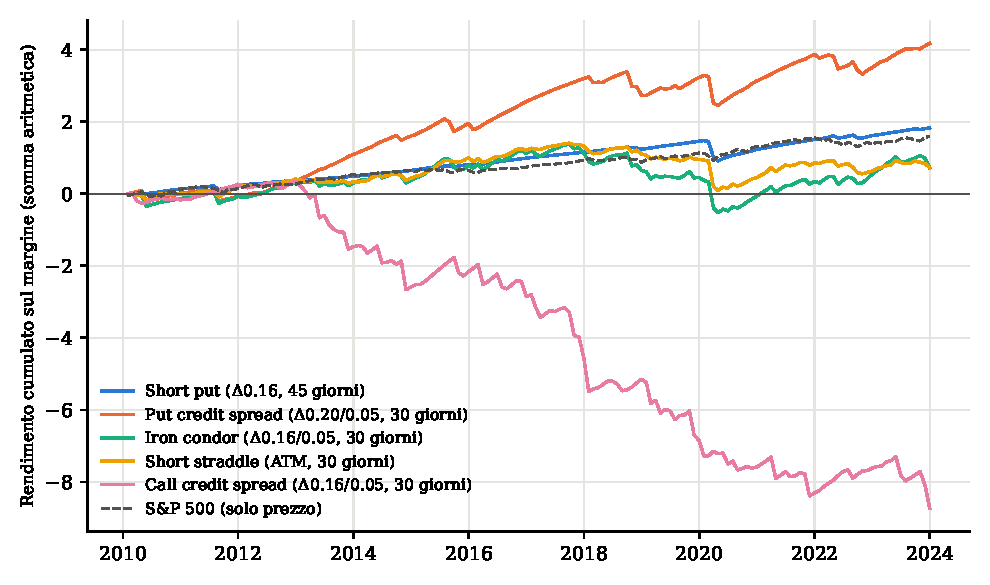
\includegraphics[width=\textwidth]{curve_it.pdf}
\caption{Rendimento cumulato sul margine (somma aritmetica dei rendimenti mensili, \emph{ladder} a capitale costante, prezzi bid-ask) per cinque configurazioni e per l'indice.}\label{fig:curve}
\end{figure}

\subsection{Rendimento e rischio delle configurazioni migliori}

La short put con delta 0{,}16 a 45 giorni chiude in utile il 94\% delle operazioni, con un risultato medio di 885 dollari per contratto e una perdita massima di 83.370 dollari: la perdita peggiore supera di oltre novanta volte il guadagno medio. Lo Sharpe è +0{,}93 ai prezzi bid-ask, superiore a quello dell'indice nel periodo (0{,}77, solo prezzo), ma il beta è 0{,}31 e l'alfa annuo, pari al +9{,}5\% del capitale a margine, ha statistica $t$ +1{,}75. Il put credit spread con delta 0{,}20 e \emph{wing} a delta 0{,}05 a 30 giorni ha Sharpe +0{,}83, beta 1{,}14 e alfa con $t$ +1{,}58; il \emph{drawdown} massimo della serie è pari al 93\% del capitale impegnato a margine, il che rende impraticabile l'impiego integrale del capitale. L'iron condor con delta 0{,}16 a 30 giorni ha Sharpe +0{,}14 e alfa con $t$ +0{,}05; lo short straddle, che è la posizione più vicina a un'esposizione pura al premio \emph{at-the-money}, ha Sharpe +0{,}18, in coerenza con un premio \emph{at-the-money} statisticamente nullo.

In sintesi, i risultati positivi coincidono con le strutture che hanno beta positivo e per le quali una parte rilevante del rendimento è esposizione al mercato azionario in un periodo in cui l'indice ha reso l'11{,}4\% annuo. È la conclusione di Israelov e Nielsen (2015) e di Jurek e Stafford (2015) applicata a queste strategie.

\subsection{Distribuzione dei rendimenti e code}\label{sec:code}

Media e Sharpe non descrivono una strategia che incassa spesso un premio piccolo e subisce raramente una perdita grande. La forma della distribuzione si misura su due livelli: per operazione, come rendimento sul margine ai prezzi bid-ask con le commissioni, e per mese, sul \emph{ladder} a capitale costante. Il riferimento è una normale con la stessa media e la stessa varianza, insieme ai rendimenti dell'indice sullo stesso orizzonte di calendario. La tabella~\ref{tab:code} riporta \emph{skewness}, \emph{excess kurtosis}, frequenza dei rendimenti inferiori alla media di oltre tre deviazioni standard rapportata a quella della normale (0{,}135\%) ed \emph{expected shortfall} all'1\% in deviazioni standard rapportato a quello della normale (2{,}665). Gli ingressi giornalieri si sovrappongono e non sono indipendenti: il test di Jarque--Bera (1987) si applica quindi solo alle serie mensili.

\begin{table}[ht]\centering\footnotesize
\caption{Forma della distribuzione dei rendimenti. Per operazione: rendimento sul margine ai prezzi bid-ask, commissioni incluse; frequenza dei rendimenti inferiori alla media di oltre tre deviazioni standard ed \emph{expected shortfall} all'1\% in deviazioni standard, entrambi rapportati alla normale; operazione peggiore in percentuale del margine. Mensile: \emph{ladder} a capitale costante; $p$-value del test di Jarque--Bera. Ultima riga: rendimenti a 30 giorni dell'S\&P 500 da ogni seduta e rendimenti mensili di prezzo.}\label{tab:code}
\resizebox{\textwidth}{!}{%
\begin{tabular}{llrrrrrrrr}\toprule
 & & \multicolumn{5}{c}{Per operazione} & \multicolumn{3}{c}{Mensile} \\ \cmidrule(lr){3-7}\cmidrule(lr){8-10}
Famiglia & Parametri & Skew. & Exc. kurt. & $<-3\sigma$ & ES 1\% & Peggiore \% & Skew. & Exc. kurt. & JB $p$ \\ \midrule
Short put & $\Delta$0{,}10, 7 gg & $-$9{,}69 & 121{,}7 & 12{,}3 & 3{,}08 & $-$40 & $-$4{,}04 & 21{,}0 & $<$0{,}001 \\
Short put & $\Delta$0{,}16, 45 gg & $-$9{,}47 & 108{,}5 & 9{,}8 & 3{,}05 & $-$125 & $-$8{,}67 & 91{,}3 & $<$0{,}001 \\
Short strangle & $\Delta$0{,}16, 30 gg & $-$8{,}01 & 101{,}7 & 8{,}4 & 2{,}57 & $-$134 & $-$7{,}67 & 78{,}0 & $<$0{,}001 \\
Put credit spread & $\Delta$0{,}20/0{,}05, 30 gg & $-$4{,}60 & 22{,}0 & 23{,}4 & 2{,}34 & $-$102 & $-$4{,}05 & 20{,}8 & $<$0{,}001 \\
Put credit spread & $\Delta$0{,}20, 1\%, 30 gg & $-$2{,}85 & 6{,}6 & 53{,}4 & 1{,}35 & $-$123 & $-$2{,}42 & 6{,}1 & $<$0{,}001 \\
Put credit spread & $\Delta$0{,}20/0{,}05, 30, TP50 gg & $-$6{,}11 & 39{,}0 & 18{,}4 & 2{,}84 & $-$102 & $-$4{,}24 & 21{,}4 & $<$0{,}001 \\
Put credit spread & $\Delta$0{,}20/0{,}05, 30, TP50/SL200 gg & $-$2{,}52 & 5{,}5 & 18{,}4 & 1{,}62 & $-$44 & $-$1{,}60 & 2{,}7 & $<$0{,}001 \\
Short straddle ATM & ATM, 30 gg & $-$2{,}92 & 23{,}9 & 8{,}3 & 2{,}03 & $-$148 & $-$4{,}20 & 33{,}1 & $<$0{,}001 \\
Iron condor & $\Delta$0{,}16/0{,}05, 30 gg & $-$2{,}82 & 9{,}7 & 16{,}7 & 2{,}00 & $-$103 & $-$2{,}57 & 11{,}0 & $<$0{,}001 \\
Iron condor & $\Delta$0{,}16, 1\%, 30 gg & $-$1{,}13 & $-$0{,}4 & 0{,}2 & 0{,}90 & $-$186 & $-$1{,}11 & 0{,}5 & $<$0{,}001 \\
Iron butterfly & ATM/$\Delta$0{,}10, 30 gg & $-$0{,}41 & $-$0{,}1 & 0{,}0 & 0{,}97 & $-$107 & $-$0{,}68 & 0{,}8 & $<$0{,}001 \\
Call credit spread & $\Delta$0{,}16/0{,}05, 30 gg & $-$1{,}99 & 2{,}6 & 1{,}9 & 1{,}12 & $-$110 & $-$1{,}89 & 3{,}0 & $<$0{,}001 \\
Long calendar ATM & ATM, 30/60 gg & 0{,}49 & $-$0{,}1 & 0{,}0 & 0{,}81 & $-$189 & $-$0{,}22 & 0{,}2 & 0{,}473 \\
Long put & $\Delta$0{,}10, 30 gg & 16{,}40 & 312{,}1 & 0{,}0 & 0{,}06 & $-$198 & 11{,}63 & 141{,}2 & $<$0{,}001 \\
\midrule
S\&P 500 & 30 gg & $-$1{,}22 & 6{,}9 & 6{,}2 & 1{,}64 & $-$34 & $-$0{,}33 & 0{,}4 & 0{,}118 \\
\bottomrule\end{tabular}}\end{table}

Le strutture che vendono volatilità senza protezione hanno code sinistre molto più lunghe di quelle della normale e dell'indice. Per la short put con delta 0{,}16 a 45 giorni la \emph{skewness} per operazione è $-$9{,}5 e l'\emph{excess kurtosis} 108, contro $-$1{,}1 e 4{,}8 per i rendimenti dell'indice a 45 giorni; le perdite oltre tre deviazioni standard sono 9{,}8 volte più frequenti che sotto la normale e l'\emph{expected shortfall} all'1\% è 3{,}0 volte quello della normale (figure~\ref{fig:code} e~\ref{fig:qq}). La forma si conserva nella serie mensile del \emph{ladder} (\emph{skewness} $-$8{,}7, \emph{excess kurtosis} 91), mentre i rendimenti mensili dell'indice nel periodo sono vicini alla normale (\emph{skewness} $-$0{,}33, \emph{excess kurtosis} 0{,}40, Jarque--Bera $p$ = 0{,}12). Sull'insieme delle 434 configurazioni, il 96\% ha \emph{skewness} per operazione negativa e il test di Jarque--Bera rifiuta la normalità della serie mensile al livello dell'1\% nel 92\% dei casi.

La coda delle perdite non è più pesante di quella dell'indice in senso asintotico. Oltre lo strike la perdita di una posizione tenuta a scadenza è lineare nel prezzo finale e ne eredita l'indice di coda: lo stimatore di Hill (1975) sui rendimenti a 30 giorni dell'indice, con il 2{,}5\% delle osservazioni nella coda, dà 2{,}9 (tra 2{,}3 e 2{,}9 con quote dall'1 al 5\%), in linea con il valore vicino a tre documentato per gli indici azionari (Gopikrishnan et al., 1999; Cont, 2001). Cambia invece il corpo della distribuzione: quasi tutti gli esiti sono concentrati sul premio incassato, la deviazione standard è piccola e le perdite rare si trovano a molte deviazioni standard di distanza. Con un indice di coda inferiore a quattro la curtosi della popolazione non è finita (Mandelbrot, 1963): i valori campionari descrivono il periodo 2010--2023 e dipendono da pochi episodi, e la parte informativa è il confronto tra strutture e con l'indice. Sui rendimenti delle strategie lo stimatore di Hill dipende dalla soglia, perché il corpo è schiacciato sul premio e le operazioni sovrapposte replicano lo stesso episodio, e non viene riportato.

\begin{figure}[ht]\centering
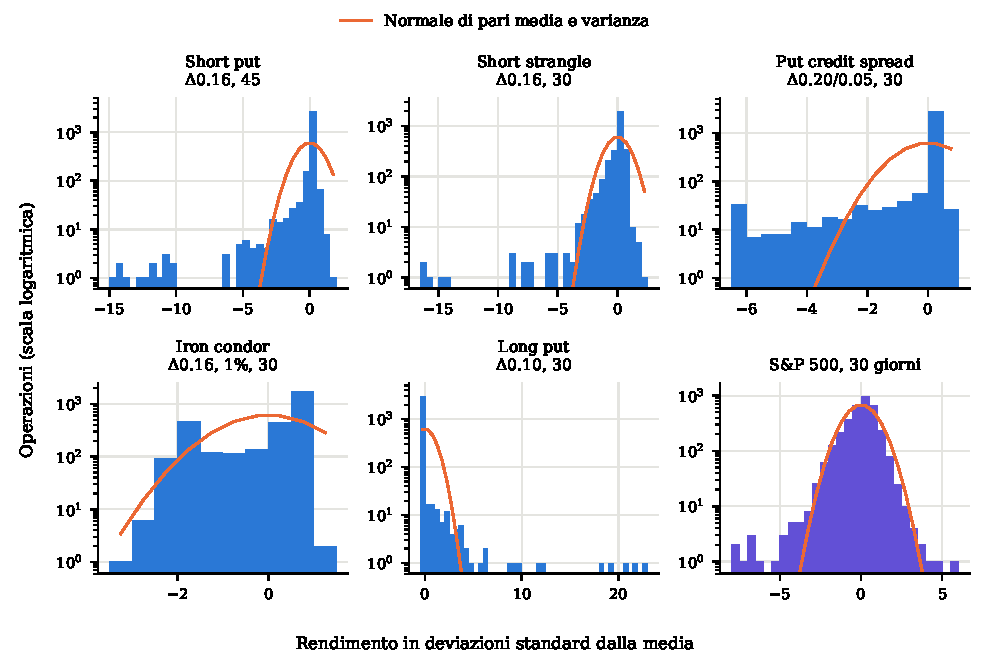
\includegraphics[width=\textwidth]{code_it.pdf}
\caption{Rendimenti per operazione in deviazioni standard dalla media, prezzi bid-ask; numero di operazioni in scala logaritmica. La curva è il numero atteso sotto una normale con la stessa media e la stessa varianza. Ultimo pannello: rendimenti a 30 giorni dell'S\&P 500 da ogni seduta.}\label{fig:code}
\end{figure}

Le strutture a rischio definito troncano la coda alla larghezza dello spread, ma il troncamento da solo non rende normale la distribuzione. Con \emph{wing} a delta 0{,}05 l'\emph{excess kurtosis} resta alta (22{,}0 per il put credit spread con delta 0{,}20, con perdite oltre tre deviazioni standard 23{,}4 volte più frequenti che sotto la normale). Con \emph{wing} all'1\% dello spot la perdita massima diventa frequente invece che rara: il 17{,}8\% delle operazioni dell'iron condor con delta 0{,}16 perde oltre il 90\% del margine, contro il 6{,}2\% sotto la normale, e l'\emph{excess kurtosis} scende a $-$0{,}39. Il rischio non è più una coda lontana ma una massa di probabilità ampia sulla perdita massima, che la curtosi non coglie. Lo \emph{stop loss} al 200\% del premio porta l'\emph{excess kurtosis} del put credit spread da 22{,}0 a 5{,}5; il costo della regola è discusso nella sottosezione seguente. Le strutture che comprano volatilità hanno la forma opposta: \emph{skewness} positiva e coda destra lunga (long put con delta 0{,}10: \emph{skewness} 16{,}4), mentre il long calendar \emph{at-the-money} 30/60 giorni è vicino alla normale (Jarque--Bera $p$ = 0{,}47 sulla serie mensile).

\begin{figure}[ht]\centering
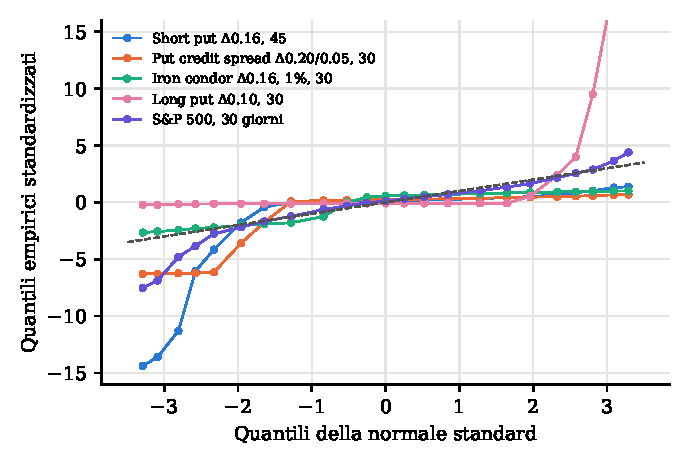
\includegraphics[width=0.7\textwidth]{qq_it.pdf}
\caption{Grafico quantile--quantile dei rendimenti per operazione standardizzati contro la normale standard; la diagonale tratteggiata corrisponde alla normale.}\label{fig:qq}
\end{figure}

Ne seguono due conseguenze. Gli ordinamenti basati su media e deviazione standard, Sharpe compreso, sopravvalutano le strutture che vendono volatilità: la vendita di opzioni \emph{out-of-the-money} è l'esempio classico di come un rendimento con \emph{skewness} negativa possa aumentare lo Sharpe senza aggiungere valore (Goetzmann et al., 2007). Il \emph{deflated Sharpe ratio} della sezione~\ref{sec:rob} corregge per \emph{skewness} e curtosi della serie mensile. Nella procedura di selezione del progetto, un criterio che divide il valore atteso per una potenza della deviazione standard eredita lo stesso limite: il rischio di coda va misurato direttamente, con l'\emph{expected shortfall} o con la probabilità della perdita massima sotto la densità GJR-GARCH, e tenuto separato dal filtro sul valore atteso.

\subsection{Regole di uscita}

Lo Sharpe mediano delle strutture a credito è +0{,}41, +0{,}44 e +0{,}43 ai prezzi mid rispettivamente per le posizioni tenute a scadenza, con \emph{take profit} al 50\% e con \emph{take profit} e \emph{stop loss} al 200\%; ai prezzi bid-ask diventa $-$0{,}05, $-$0{,}44 e $-$0{,}73. Ai prezzi mid le regole di uscita non modificano il rendimento atteso, come deve essere per una regola che non contiene informazione; ai prezzi bid-ask lo peggiorano, perché ogni chiusura anticipata paga un secondo spread, mentre il \emph{cash settlement} a scadenza non ne paga. Le regole riducono il \emph{drawdown} massimo, ma a un costo certo.

\subsection{Filtri di ingresso}

La Tabella~\ref{tab:filt} confronta, dal 2012, lo Sharpe mediano senza filtri con quello ottenuto aprendo posizioni soltanto quando la volatilità implicita supera la previsione GARCH, soltanto quando è inferiore, e nei terzili estremi del livello di volatilità implicita. Il filtro $\sigma_{\mathrm{ATM}}>\sigma_{\mathrm{GARCH}}$ migliora lo Sharpe nell'86\% delle configurazioni a credito, e la mediana passa da $-$0{,}26 a $-$0{,}05. Il miglioramento è sistematico nel segno ma non trasforma le famiglie in perdita in famiglie in utile. Per la short put con delta 0{,}16 a 45 giorni lo Sharpe passa da +0{,}90 a +1{,}62; per l'iron condor con delta 0{,}16 a 30 giorni da +0{,}18 a +0{,}70. Il risultato va letto insieme a quello della Sezione~\ref{sec:vrp}: il segnale ha il segno corretto, ma la sua significatività statistica sul premio è debole e il filtro è stato valutato sullo stesso campione su cui è stato concepito.

\begin{table}[ht]\centering\small
\caption{Sharpe mediano per famiglia e per filtro di ingresso, prezzi bid-ask, 2012--2023. I mesi senza operazioni contano come rendimento nullo.}\label{tab:filt}
\begin{tabular}{lrrrrrr}\toprule
Famiglia & $N$ & Nessuno & IV $>$ GARCH & IV $\le$ GARCH & IV alta & IV bassa \\ \midrule
Short put & 48 & +0{,}88 & +0{,}92 & +0{,}56 & +0{,}83 & +0{,}28 \\
Short strangle & 48 & +0{,}43 & +0{,}70 & +0{,}15 & +0{,}37 & +0{,}21 \\
Put credit spread & 96 & +0{,}13 & +0{,}24 & $-$0{,}04 & +0{,}24 & $-$0{,}04 \\
Short straddle ATM & 12 & +0{,}20 & +0{,}41 & $-$0{,}00 & +0{,}20 & +0{,}04 \\
Iron condor & 96 & $-$0{,}85 & $-$0{,}40 & $-$0{,}83 & $-$0{,}55 & $-$0{,}30 \\
Iron butterfly & 24 & $-$0{,}25 & $-$0{,}06 & $-$0{,}32 & $-$0{,}14 & $-$0{,}10 \\
Call credit spread & 96 & $-$1{,}27 & $-$0{,}83 & $-$1{,}02 & $-$1{,}00 & $-$0{,}55 \\
\bottomrule\end{tabular}\end{table}

\subsection{Filtro operativo sulla volatilità realizzata}\label{sec:fvol}

Una regola prudenziale diffusa consiste nel sospendere le nuove operazioni quando la volatilità realizzata è eccessiva e nel riprenderle quando rientra, con l'obiettivo di evitare gli eventi estremi. La regola è stata verificata su tutte le configurazioni a credito: gli ingressi sono sospesi quando la volatilità storica a 21 sedute (HV21) supera una soglia e riprendono quando torna al di sotto; le posizioni già aperte seguono la propria gestione. Le soglie sono il 20\%, il 25\% e il 30\% annualizzato e il 90° percentile calcolato sui soli dati già osservati (Tabella~\ref{tab:fvol}).

\begin{table}[ht]\centering\small
\caption{Sospensione degli ingressi in funzione della volatilità realizzata: mediane sulle configurazioni a credito, prezzi bid-ask, marzo 2011--dicembre 2023. \emph{Drawdown} e mese peggiore in percentuale del capitale impegnato a margine.}\label{tab:fvol}
\begin{tabular}{lrrrrrr}\toprule
 & Operazioni & Sharpe & Sharpe & \emph{Drawdown} & \emph{Drawdown} & Mese \\
Filtro & eseguite \% & mediano & migliore \% & mediano \% & minore \% & peggiore \% \\ \midrule
Nessun filtro & 100 & $-$0{,}30 & -- & 393 & -- & $-$69 \\
HV21 $\le$ 20\% & 82 & $-$0{,}37 & 49 & 324 & 85 & $-$64 \\
HV21 $\le$ 25\% & 91 & $-$0{,}34 & 45 & 343 & 82 & $-$65 \\
HV21 $\le$ 30\% & 97 & $-$0{,}30 & 46 & 370 & 73 & $-$67 \\
HV21 $\le$ 90° percentile & 90 & $-$0{,}35 & 42 & 356 & 80 & $-$65 \\
HV10 $\le$ 25\% & 91 & $-$0{,}36 & 38 & 377 & 69 & $-$65 \\
Solo HV21 $>$ 25\% & 9 & +0{,}07 & 76 & 55 & 100 & $-$31 \\
\bottomrule\end{tabular}\end{table}

I risultati sono tre. Primo: il filtro non migliora il rendimento corretto per il rischio. Con la soglia del 25\% lo Sharpe mediano passa da $-$0{,}30 a $-$0{,}34 e migliora soltanto nel 45\% delle configurazioni; per la short put con delta 0{,}16 a 45 giorni scende da +0{,}89 a +0{,}64, per l'iron condor con delta 0{,}16 a 30 giorni da +0{,}17 a +0{,}08. Secondo: il \emph{drawdown} si riduce nell'82\% delle configurazioni, ma in misura vicina alla riduzione del numero di operazioni (91\% di quelle senza filtro), e il mese peggiore non cambia: per la short put resta pari al 43{,}9\% del capitale a margine con e senza filtro. Le posizioni che hanno subito le perdite maggiori, nel febbraio 2020, erano state aperte con volatilità realizzata bassa: il filtro sospende gli ingressi dopo l'evento, non prima. Terzo: le operazioni aperte con HV21 superiore al 25\% hanno un rendimento medio per operazione superiore alla media (per la short put 5{,}2\% del margine contro 1{,}8\%), sicché il filtro rinuncia proprio alle operazioni meglio remunerate.

\begin{table}[ht]\centering\small
\caption{Premio successivo a 30 giorni per livello della volatilità storica a 21 sedute all'ingresso. Valori in punti di volatilità.}\label{tab:hv}
\begin{tabular}{lrrrrrrrrr}\toprule
HV21 (\%) & Sedute & IV ATM & Real. & ATM $-$ real. & $t$ & MF $-$ real. & \% $>0$ & 5° perc. & Min. \\ \midrule
$\le$ 10 & 998 & 10{,}79 & 11{,}01 & $-$0{,}22 & $-$0{,}44 & +2{,}36 & 61 & $-$10{,}2 & $-$21 \\
10--15 & 1.041 & 13{,}77 & 12{,}72 & +1{,}05 & 1{,}47 & +3{,}56 & 77 & $-$5{,}8 & $-$77 \\
15--20 & 529 & 17{,}26 & 15{,}71 & +1{,}55 & 1{,}85 & +4{,}35 & 72 & $-$9{,}2 & $-$72 \\
20--25 & 269 & 20{,}91 & 19{,}69 & +1{,}21 & 1{,}05 & +4{,}47 & 67 & $-$9{,}3 & $-$70 \\
25--30 & 176 & 24{,}09 & 22{,}50 & +1{,}58 & 1{,}43 & +4{,}75 & 66 & $-$6{,}9 & $-$68 \\
$>$ 30 & 115 & 33{,}14 & 33{,}45 & $-$0{,}31 & $-$0{,}10 & +3{,}63 & 68 & $-$42{,}0 & $-$68 \\
\bottomrule\end{tabular}\end{table}

La Tabella~\ref{tab:hv} mostra la ragione. Il premio \emph{at-the-money} successivo non diminuisce quando la volatilità realizzata è alta: è prossimo a zero nelle due classi estreme ($-$0{,}22 punti con HV21 inferiore al 10\%, $-$0{,}31 punti oltre il 30\%) e positivo nelle classi intermedie. Le perdite estreme hanno origine nelle fasi di calma: il valore minimo del premio appartiene alla classe 10--15\%. Oltre il 30\% la dispersione è molto ampia e il campione ridotto, e nessuna delle medie per classe è statisticamente diversa da zero.

Il filtro è inoltre ridondante rispetto alla costruzione delle strategie. Gli strike sono scelti per delta sulla volatilità implicita di mercato, sicché la struttura si allarga da sola quando la volatilità sale: la distanza dal forward della put con delta 0{,}16 a 30 giorni è in media il 3{,}8\% nel terzile di volatilità implicita bassa (IV media 10{,}0\%), il 5{,}0\% nel terzile intermedio e il 7{,}5\% nel terzile alto (IV media 22{,}2\%), con correlazione 0{,}98 tra distanza e volatilità implicita. Nella procedura di selezione del progetto la densità GJR-GARCH svolge la stessa funzione sul valore atteso e sulle probabilità: una volatilità prevista più alta allarga la distribuzione e sposta la selezione verso strutture più larghe o la esclude. La volatilità è quindi già incorporata due volte, nel posizionamento degli strike e nel filtro sul valore atteso.

La conclusione operativa è che una sospensione basata sulla volatilità realizzata non è necessaria e non protegge dagli eventi estremi, che per definizione sopraggiungono da condizioni di calma. Equivale a una riduzione dell'esposizione, ottenibile in modo più diretto con la quota di capitale impegnata a margine; la protezione dalle code è affidata al rischio definito delle strutture e al dimensionamento.

\section{Robustezza e multiple testing}\label{sec:rob}

\subsection{Il costo di esecuzione}

Su 434 configurazioni lo Sharpe mediano è +0{,}39 ai prezzi mid e $-$0{,}40 ai prezzi bid-ask; la quota di configurazioni con Sharpe positivo scende dal 64\% al 38\% (Figura~\ref{fig:sharpe}). Il prezzo effettivo di esecuzione è compreso tra i due estremi: le quotazioni di chiusura sovrastimano lo spread tipico delle ore centrali, ma un ordine al prezzo mid su una struttura a più gambe non ha garanzia di esecuzione. Il sito consente di fissare la quota di spread pagata e ricalcola ogni statistica.

\begin{figure}[ht]\centering
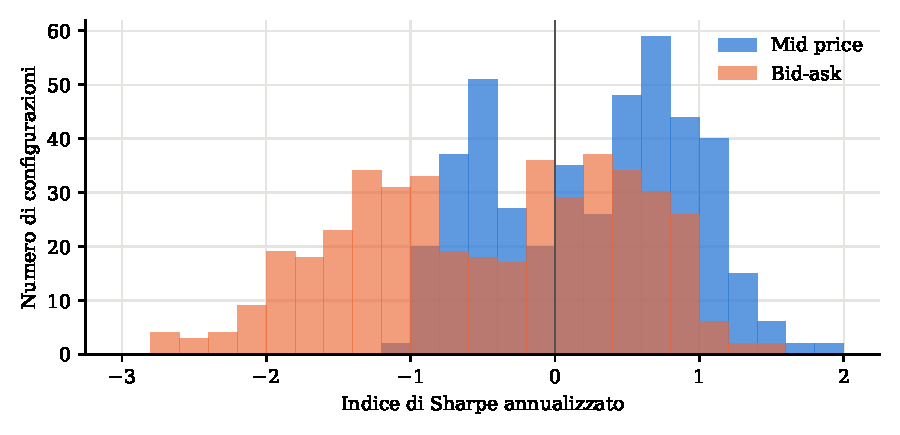
\includegraphics[width=0.54\textwidth]{sharpe_it.pdf}\hfill
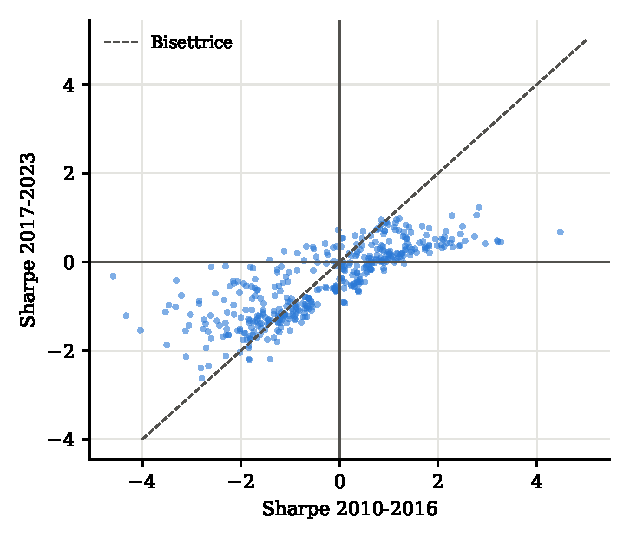
\includegraphics[width=0.42\textwidth]{meta_it.pdf}
\caption{A sinistra: distribuzione dello Sharpe sulle 434 configurazioni, ai prezzi mid e bid-ask. A destra: Sharpe nel 2010--2016 e nel 2017--2023 per le configurazioni a credito.}\label{fig:sharpe}
\end{figure}

\subsection{Alfa rispetto all'indice}

La quota di configurazioni con alfa positivo e statistica $t$ superiore a 2 è il 16{,}4\% ai prezzi mid e il 2{,}5\% ai prezzi bid-ask. Sotto l'ipotesi nulla di alfa pari a zero per tutte le configurazioni, la quota attesa per solo effetto del caso è il 2{,}5\%. Il 49{,}8\% delle configurazioni ha invece alfa significativamente negativo ai prezzi bid-ask. Ai prezzi effettivamente negoziabili l'evidenza di \emph{extra return} rispetto all'esposizione azionaria non si distingue da quella attesa in assenza di qualunque premio incassabile.

\subsection{Selezione a posteriori}

Tra 434 configurazioni la migliore ha Sharpe 1{,}58. Il massimo atteso sotto l'ipotesi nulla, calcolato secondo Bailey e López de Prado (2014) dalla dispersione degli Sharpe osservati, è 2{,}85; il \emph{deflated Sharpe ratio} della configurazione migliore è 0{,}012. La misura è prudenziale, perché la dispersione include differenze effettive tra famiglie e le prove non sono indipendenti; indica comunque che il valore massimo osservato non costituisce, da solo, evidenza di un rendimento atteso positivo.

Una verifica più diretta è la divisione del campione. La correlazione di rango tra lo Sharpe nel 2010--2016 e nel 2017--2023 è 0{,}84: l'ordinamento tra famiglie è stabile. Il livello non lo è: le venti configurazioni migliori nel primo periodo hanno Sharpe medio 2{,}67 nel primo e 0{,}60 nel secondo, mentre la mediana di tutte le configurazioni a credito nel secondo periodo è $-$0{,}44. Un parametro scelto sul passato conserva la posizione relativa e perde circa tre quarti del risultato.

\section{Verifiche sul codice preesistente}\label{sec:codice}

La ricostruzione ha richiesto la lettura del codice del repository del gruppo. Si riportano i punti che modificano i risultati numerici, con il file interessato.

\begin{enumerate}
\item \texttt{vrp\_analysis.py} e \texttt{utils\_vrp\_analysis.py}. La volatilità realizzata ``futura'' è calcolata con \texttt{rets.shift(-1).rolling(window=dte).std()}. La finestra mobile è rivolta al passato: l'espressione usa i rendimenti da $t-\mathrm{dte}+2$ a $t+1$, cioè la volatilità trascorsa spostata di una seduta. I grafici ``IV meno RV futura'' confrontano quindi l'implicita con la realizzata passata. La forma corretta è \texttt{rets.rolling(n).std().shift(-n)}, con $n$ espresso in sedute.
\item Negli stessi file e in \texttt{utils\_forecast\_price\_distribution.py} la vita residua in giorni di calendario è usata come numero di sedute. Per un'opzione a 20 giorni di calendario la previsione cumula 20 varianze giornaliere invece di circa 14, e la deviazione standard della distribuzione prevista risulta sovrastimata di un fattore $\sqrt{20/14}\approx 1{,}20$. L'effetto è una sottostima sistematica del valore atteso delle strutture vendute.
\item In \texttt{utils\_forecast\_price\_distribution.py} i prezzi sono scaricati fino alla data di scadenza e la stima usa i dati fino a $h$ sedute prima dell'ultima: per $h=20$ la finestra termina circa sei sedute prima della data di ingresso, e il prezzo di partenza della distribuzione non è quello di ingresso. Non vi è uso di informazioni future, ma previsione e operazione non sono allineate.
\item In \texttt{generate\_signal\_garch\_vs\_iv.py} il ramo che dovrebbe generare il segnale di acquisto di volatilità (\texttt{spread <= -0.01}) è preceduto dal ramo \texttt{spread < 0.00} e non viene mai eseguito.
\item In \texttt{utils\_criteria.py} l'argomento \texttt{payoff} è sovrascritto all'inizio della funzione da un vettore di prova; i criteri restituiti non dipendono dalla strategia passata.
\item Il file \texttt{.gitattributes} della branch principale di sviluppo contiene una riga non valida, residuo di un conflitto di fusione, e la quota Git LFS del repository è esaurita: i file \texttt{.pkl} e \texttt{.csv} non sono più scaricabili. Le analisi di questo documento partono dagli archivi compressi originali, che sono nel repository senza LFS.
\end{enumerate}

Il risultato storico del gruppo sull'iron condor a 10 giorni (rendimento annualizzato dell'1{,}85\%, quota di operazioni in utile del 57{,}3\%, \emph{drawdown} massimo superiore alla metà del capitale) è coerente, per segno e ordine di grandezza, con i risultati ottenuti qui per la stessa famiglia.

\section{Limiti}\label{sec:limiti}

\emph{Dati.} Le quotazioni sono di fine giornata; lo spread alla chiusura è più ampio di quello tipico della seduta e i prezzi di chiusura di opzioni e indice possono non essere sincroni. Le scadenze mensili \emph{AM-settled} sono valutate alla chiusura del giorno di scadenza. Il campione copre quattordici anni di mercato prevalentemente in rialzo.

\emph{Margine.} Il margine delle posizioni scoperte è approssimato con il 20\% del nozionale; il margine effettivo dipende dal broker e dal regime, e in condizioni di stress aumenta nel momento in cui la posizione perde. Le serie non includono il rendimento della liquidità a garanzia.

\emph{Disegno.} Ogni seduta apre una posizione unitaria, senza dimensionamento dinamico. La serie mensile attribuisce il risultato al mese di chiusura e non valuta le posizioni aperte ai prezzi di mercato: il \emph{drawdown} massimo infra-mensile è sottostimata. L'alfa è stimato rispetto al solo indice.

\emph{Selezione.} Le famiglie e i parametri sono quelli che il progetto ha esplorato negli anni sullo stesso archivio: nessuna parte del campione è realmente \emph{out-of-sample}. La sola verifica non contaminata è la registrazione dei segnali prima che l'esito sia noto.

\section{Conclusioni}\label{sec:concl}

Sulle \emph{option chain} SPX dal 2010 al 2023 il premio per il rischio di volatilità esiste nella forma descritta dalla letteratura: la varianza implicita \emph{model-free} supera la realizzata in misura ampia e significativa, le put \emph{out-of-the-money} hanno restituito ai compratori circa la metà del premio, e la distribuzione del premio realizzato è dominata da pochi eventi estremi. Non esiste invece, nel campione, un premio significativo sulla volatilità \emph{at-the-money} oltre le due settimane: a quel livello la volatilità implicita è una previsione non distorta di quella realizzata e batte sia il modello GARCH sia la volatilità storica. Il mercato appare efficiente sul piano informativo nel centro della superficie e remunera un rischio di coda sulle \emph{wing}.

Per le strategie del progetto le conseguenze sono tre. La prima: le strutture simmetriche a rischio definito, in particolare l'iron condor, vendono insieme la parte della superficie che contiene il premio (le put) e quella che non lo contiene (le call), e pagano lo spread su quattro gambe; il risultato netto è nullo o negativo. La seconda: le strutture che vendono put conservano un risultato positivo anche dopo i costi, ma una parte rilevante è esposizione al mercato azionario e l'alfa residuo non è statisticamente distinguibile da zero nella grande maggioranza delle configurazioni. La terza: regole di uscita e filtri modificano la distribuzione dei risultati ma non creano rendimento atteso; la sospensione degli ingressi quando la volatilità realizzata è elevata riduce l'esposizione senza evitare gli eventi estremi, perché gli strike scelti per delta si allargano già con la volatilità implicita; il filtro basato sul confronto con il GARCH ha il segno corretto e merita una verifica prospettica.

La distribuzione dei rendimenti qualifica ogni Sharpe riportato in questo lavoro. Le strutture che vendono volatilità hanno, per operazione, \emph{skewness} molto più negativa e curtosi molto più alta di quelle dell'indice, e la serie mensile non è normale nel 92\% delle configurazioni: il rischio di coda va misurato direttamente e non dedotto dalla deviazione standard.

L'ipotesi di lavoro secondo cui il premio esiste ma il tentativo di incassarlo in modo sistematico tende, nel lungo periodo e al netto dei costi, a un risultato nullo non è rifiutata dai dati.

\appendix
\section{Payoff a scadenza delle strutture}\label{app:payoff}

Con $S_T$ il valore dell'indice a scadenza e i premi espressi in punti indice, i payoff per unità sono i seguenti. Short put di strike $B$ e premio $P_B$: $P_B - \max(B-S_T,0)$. Put credit spread con strike $A<B$: credito $c=P_B-P_A$, payoff $c - \max(B-S_T,0) + \max(A-S_T,0)$, perdita massima $(B-A)-c$, \emph{breakeven} $B-c$. Iron condor con strike $A<B<C<D$: credito $c=(P_B+C_C)-(P_A+C_D)$, payoff
\[
c - \max(B-S_T,0) + \max(A-S_T,0) - \max(S_T-C,0) + \max(S_T-D,0),
\]
perdita massima $\max(B-A,\,D-C)-c$, punti di pareggio $B-c$ e $C+c$. L'iron butterfly è il caso $B=C$. Per il calendar su put di strike $K$, venduta sulla scadenza $T_1$ e comprata sulla scadenza $T_2>T_1$, il risultato alla prima scadenza è $P(K,T_2;T_1) - \max(K-S_{T_1},0) - d$, con $d$ il debito iniziale e $P(K,T_2;T_1)$ il valore di mercato della gamba superstite in $T_1$. Tutti i valori in dollari si ottengono moltiplicando per 100.

\begin{thebibliography}{99}\small
\bibitem{} Bailey, D. H. e López de Prado, M. (2014). The deflated Sharpe ratio: correcting for selection bias, backtest overfitting, and non-normality. \emph{Journal of Portfolio Management}, 40(5), 94--107.
\bibitem{} Bakshi, G. e Kapadia, N. (2003). Delta-hedged gains and the negative market volatility risk premium. \emph{Review of Financial Studies}, 16(2), 527--566.
\bibitem{} Bates, D. S. (2000). Post-'87 crash fears in the S\&P 500 futures option market. \emph{Journal of Econometrics}, 94(1--2), 181--238.
\bibitem{} Beckmeyer, H., Branger, N. e Gayda, L. (2023). Retail traders love 0DTE options... but should they? Working paper, SSRN.
\bibitem{} Black, F. (1976). The pricing of commodity contracts. \emph{Journal of Financial Economics}, 3(1--2), 167--179.
\bibitem{} Black, F. e Scholes, M. (1973). The pricing of options and corporate liabilities. \emph{Journal of Political Economy}, 81(3), 637--654.
\bibitem{} Bollen, N. P. B. e Whaley, R. E. (2004). Does net buying pressure affect the shape of implied volatility functions? \emph{Journal of Finance}, 59(2), 711--753.
\bibitem{} Bollerslev, T. (1986). Generalized autoregressive conditional heteroskedasticity. \emph{Journal of Econometrics}, 31(3), 307--327.
\bibitem{} Bollerslev, T., Tauchen, G. e Zhou, H. (2009). Expected stock returns and variance risk premia. \emph{Review of Financial Studies}, 22(11), 4463--4492.
\bibitem{} Bollerslev, T. e Todorov, V. (2011). Tails, fears, and risk premia. \emph{Journal of Finance}, 66(6), 2165--2211.
\bibitem{} Bondarenko, O. (2014). Why are put options so expensive? \emph{Quarterly Journal of Finance}, 4(3), 1450015.
\bibitem{} Britten-Jones, M. e Neuberger, A. (2000). Option prices, implied price processes, and stochastic volatility. \emph{Journal of Finance}, 55(2), 839--866.
\bibitem{} Broadie, M., Chernov, M. e Johannes, M. (2009). Understanding index option returns. \emph{Review of Financial Studies}, 22(11), 4493--4529.
\bibitem{} Canina, L. e Figlewski, S. (1993). The informational content of implied volatility. \emph{Review of Financial Studies}, 6(3), 659--681.
\bibitem{} Carr, P. e Wu, L. (2009). Variance risk premiums. \emph{Review of Financial Studies}, 22(3), 1311--1341.
\bibitem{} Christensen, B. J. e Prabhala, N. R. (1998). The relation between implied and realized volatility. \emph{Journal of Financial Economics}, 50(2), 125--150.
\bibitem{} Constantinides, G. M., Jackwerth, J. C. e Savov, A. (2013). The puzzle of index option returns. \emph{Review of Asset Pricing Studies}, 3(2), 229--257.
\bibitem{} Cont, R. (2001). Empirical properties of asset returns: stylized facts and statistical issues. \emph{Quantitative Finance}, 1(2), 223--236.
\bibitem{} Coval, J. D. e Shumway, T. (2001). Expected option returns. \emph{Journal of Finance}, 56(3), 983--1009.
\bibitem{} Dew-Becker, I. e Giglio, S. (2023). Risk preferences implied by synthetic options. NBER Working Paper 31833.
\bibitem{} Dew-Becker, I. e Giglio, S. (2025). The decline of the variance risk premium: evidence from traded and synthetic options. Federal Reserve Bank of Chicago, Working Paper 2025-17.
\bibitem{} Dew-Becker, I., Giglio, S., Le, A. e Rodriguez, M. (2017). The price of variance risk. \emph{Journal of Financial Economics}, 123(2), 225--250.
\bibitem{} Engle, R. F. (1982). Autoregressive conditional heteroscedasticity with estimates of the variance of United Kingdom inflation. \emph{Econometrica}, 50(4), 987--1007.
\bibitem{} Fama, E. F. (1970). Efficient capital markets: a review of theory and empirical work. \emph{Journal of Finance}, 25(2), 383--417.
\bibitem{} Gârleanu, N., Pedersen, L. H. e Poteshman, A. M. (2009). Demand-based option pricing. \emph{Review of Financial Studies}, 22(10), 4259--4299.
\bibitem{} Glosten, L. R., Jagannathan, R. e Runkle, D. E. (1993). On the relation between the expected value and the volatility of the nominal excess return on stocks. \emph{Journal of Finance}, 48(5), 1779--1801.
\bibitem{} Goetzmann, W., Ingersoll, J., Spiegel, M. e Welch, I. (2007). Portfolio performance manipulation and manipulation-proof performance measures. \emph{Review of Financial Studies}, 20(5), 1503--1546.
\bibitem{} Gopikrishnan, P., Plerou, V., Amaral, L. A. N., Meyer, M. e Stanley, H. E. (1999). Scaling of the distribution of fluctuations of financial market indices. \emph{Physical Review E}, 60(5), 5305--5316.
\bibitem{} Hill, B. M. (1975). A simple general approach to inference about the tail of a distribution. \emph{Annals of Statistics}, 3(5), 1163--1174.
\bibitem{} Ilmanen, A. (2012). Do financial markets reward buying or selling insurance and lottery tickets? \emph{Financial Analysts Journal}, 68(5), 26--36.
\bibitem{} Israelov, R. e Nielsen, L. N. (2015). Covered calls uncovered. \emph{Financial Analysts Journal}, 71(6), 44--57.
\bibitem{} Jackwerth, J. C. (2000). Recovering risk aversion from option prices and realized returns. \emph{Review of Financial Studies}, 13(2), 433--451.
\bibitem{} Jarque, C. M. e Bera, A. K. (1987). A test for normality of observations and regression residuals. \emph{International Statistical Review}, 55(2), 163--172.
\bibitem{} Jiang, G. J. e Tian, Y. S. (2005). The model-free implied volatility and its information content. \emph{Review of Financial Studies}, 18(4), 1305--1342.
\bibitem{} Jurek, J. W. e Stafford, E. (2015). The cost of capital for alternative investments. \emph{Journal of Finance}, 70(5), 2185--2226.
\bibitem{} Mandelbrot, B. (1963). The variation of certain speculative prices. \emph{Journal of Business}, 36(4), 394--419.
\bibitem{} Mincer, J. e Zarnowitz, V. (1969). The evaluation of economic forecasts. In J. Mincer (a cura di), \emph{Economic Forecasts and Expectations}. NBER.
\bibitem{} Newey, W. K. e West, K. D. (1987). A simple, positive semi-definite, heteroskedasticity and autocorrelation consistent covariance matrix. \emph{Econometrica}, 55(3), 703--708.
\bibitem{} Poon, S.-H. e Granger, C. W. J. (2003). Forecasting volatility in financial markets: a review. \emph{Journal of Economic Literature}, 41(2), 478--539.
\bibitem{} Santa-Clara, P. e Saretto, A. (2009). Option strategies: good deals and margin calls. \emph{Journal of Financial Markets}, 12(3), 391--417.
\bibitem{} Todorov, V. (2010). Variance risk-premium dynamics: the role of jumps. \emph{Review of Financial Studies}, 23(1), 345--383.
\end{thebibliography}
\end{document}
